\documentclass[a4paper,12pt]{article}
\usepackage{graphicx}

\begin{document}
El proyecto Moogle está constituido por 2 clases principales, MoogleEngine y MoogleServer. 
En este informe me centraré en explicar la constitución y el funcionamiento de la clase 
MoogleEngine. Dicha clase contiene otras 6 clases en su interior(Moogle, Load, Matriz, 
Consulta, SearchItem, SearchResult), las cuales correctamente concatenadas conllevan al 
funcionamiento de Moogle. En el siguiente diagrama explicaré dicha composición. 
\begin{figure}[h]
    \includegraphics*{Grafico 1.png}
    \end{figure}       
    \section*{}
        Para lograr una correcta comprensión de este proyecto e informe, explicaré a profundidad 
cada clase incorporada, con lo cual me refiero a las siguientes: Load, Matriz, Consulta. A 
continuación comenzare a abordar la clase Load.
La clase Load, pública y estática, está constituida por los siguientes campos o atributos de 
clases, y funciones o métodos, los cuales son:
\subsection*{Campos o Atributos:}
\begin{itemize}
    \item private static string [] path=Directory.GetFiles(Path.Join("..","Content",""));
    \item private static string [][] text=new string[title.Length][];  
    \item private static string[] title= new string[path.Length]; 
    
\end{itemize}
\subsection*{Métodos o Funciones:}
\begin{itemize}
    \item  public static void run (); 
    \item public static string EliminarTildes( string texto);
    \item public static string EliminarCaracteres(string texto);
    \item public static string[][] GetText();
    \item public static string[] GetTitle();
    \item public static string [] GetPath();
    
\end{itemize}
La función principal de esta clase es cargar y modificar toda la base de datos (compuesta por 
archivos .txt), mediante el método run().Dentro de este método se le asignan valores a todos 
los campos de clase excepto al path, y se realiza una llamada a los métodos 
EliminarTildes(string texto), EliminarCaracteres(string texto), los cuales modifican 
correspondientemente todos los archivos .txt, el primero realiza lo que su propio nombre 
indica y además deja el texto en letra minúscula, el segundo elimina todos los caracteres
especiales dentro del texto, dejando solo las letras del alfabeto y los números, todo esto 
dentro de un ciclo for. El propósito de la creación de los métodos, GetText(), GetTitle(), 
GetPath(), radica en obtener los valores de los campos privados text, title, path, para su 
posterior utilización. He aquí dicho método principal run();
\begin{figure}[h]
    \includegraphics*{Code 1.png}
    
\end{figure} 
\subsection*{}
A continuación un mapa conceptual, el cual explica todo lo antes 
mencionado de una forma resumida e intuitiva.

\begin{figure}[h]
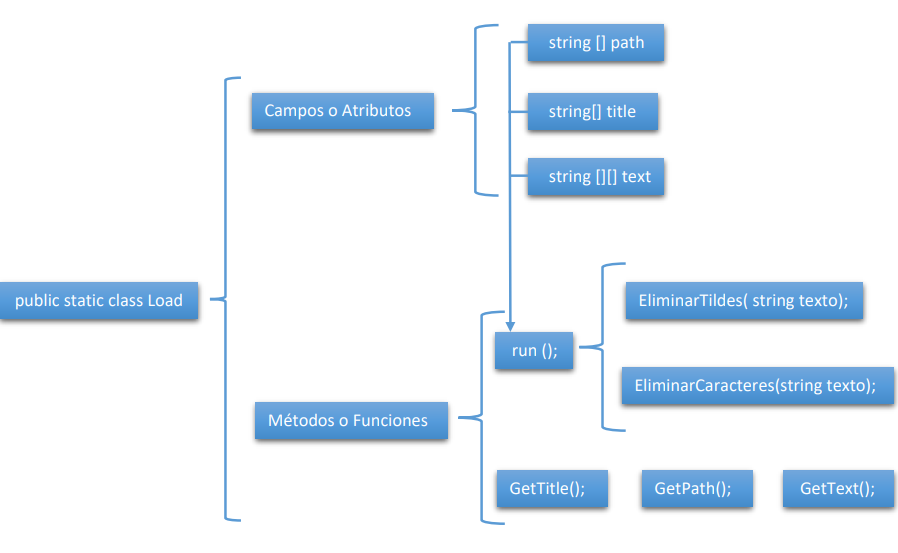
\includegraphics[width=17cm]{Grafico 2.png}
\end{figure}
\section*{Clase Matriz}
La clase Matriz, pública y estática, se encarga de todo lo relacionado con la creación del 
modelo vectorial, o sea, con la vectorización de todos los documentos de la base de datos. 
Dicha clase está compuesta por los campos y métodos de clases siguientes:
\subsection*{Campos o Atributos:}
\begin{itemize}
    \item  public static List ListDiccionarios;
    \item public static List ListDiccionariosTF;  
     \end{itemize}
     \subsection*{Métodos o Funciones:}
     \begin{itemize}
         \item private static void Diccionario();
         \item public static void DiccionarioTF();
         \item public static float Tf (float repeticion, float cantPalabras );
         \item public static float Idf (float TotalDocumentos, float documentos);
        \end{itemize}
        \subsection*{Otros Métodos Algebraicos:}
        \begin{itemize}
            \item public static int [,] MultiplicarEscalar(int[,]a,int k); (El cual puede ser usado para 
            multiplicar una matriz por un escalar)
            \item public static int[,] Traspuesta(int[,]a); (El cual puede ser usado para hallar la matriz 
            traspuesta)
            \item public static int[,] Sumar(int[,]a,int[,]b); (Para sumar dos matrices)
            \item public static int[,] Restar(int[,]a,int[,]b); (Para restar dos matrices)
            \item static int[,] Multiplicar(int[,]a,int[,]b); (Para multiplicar dos matrices)
        \end{itemize}
        El método principal de esta clase ( DiccionarioTF();) , es el encargado de la creación del modelo 
vectorial de los documentos. Para esto, se auxilia, llamando al método Diccionario(); , el cual 
crea una serie de diccionarios en los que la llave(string) son las palabras de un documento x y 
el valor(int), la cantidad de veces que se repite una palabra en dicho documento, para 
posteriormente poder ser utilizados para el cálculo del Tf de dicha palabra. Estos son 
almacenados en el campo de clase (ListDiccionarios), para más adelante tener acceso a todos. 
Al tener ya creados estos diccionarios, el método (DiccionarioTF();), dentro de dos ciclos for, 
crea otras series de diccionarios, los cuales tienen por llave(string) las palabras de un 
documento x y el valor(float), el TF de una palabra en este documento, el cual es calculado a 
través de la función (float Tf (float repeticion,float cantPalabras );) y con los valores de 
(ListDiccionarios). TF-IDF, se refiere a una técnica de vectorizacion de documentos. El Tf-idf, 
frecuencia de término – frecuencia inversa de documento (o sea, la frecuencia de ocurrencia 
del término en la colección de documentos), es una medida numérica que expresa cuán 
relevante es una palabra para un documento en una colección. El valor tf-idf aumenta 
proporcionalmente al número de veces que una palabra aparece en el documento, pero es compensada por la frecuencia de la palabra en la colección de documentos, lo que permite 
manejar el hecho de que algunas palabras son generalmente más comunes que otras. El tf se 
obtiene a través de la división del número de veces que aparece un término en un 
documento con la cantidad de términos contenidos en dicho documento. El idf se obtiene 
dividiendo el número total de documentos por el número de documentos que contienen el 
término, y se toma el logaritmo de ese cociente. Estos diccionarios son almacenados dentro 
del campo de clase (ListDiccionariosTF), para tener acceso completo a ellos. El método (float 
Idf (float TotalDocumentos,float documentos);) es utilizado posteriormente en la clase 
Consulta, para el cálculo del IDF de los términos. A continuación será visible para su total 
comprensión el método (DiccionarioTF();).
\begin{figure}[h]
    \includegraphics*{code 2.png}
    \end{figure}
\subsection*{}
*Nótese que por cada documento, se crea un Diccionariotf(string, float).
\linebreak
\linebreak
A continuación un grafico donde se puede apreciar la composición de dicha clase Matriz
\subsection*{}
\begin{figure}[h] 
    \includegraphics*[width=17cm]{grafico 3.png}
    
\end{figure}

\newpage
\section*{Clase Consulta}

La clase Consulta, pública y estática, es la encargada de realizar las operaciones de Tf-Idf 
restantes y modificar el query, introducido por el usuario, de igual forma como se modificó la 
base de datos, a través de los métodos EliminarTildes(); y EliminarCaracteres();. Esta clase 
cuenta con los siguientes campos y métodos:
\subsection*{Campos o Atributos:}
\begin{itemize}
    \item public static string [] busqueda;
\item public static float [] idf;
\item public static float[] score =new float[Matriz.ListDiccionariosTF.Count]; 
    \item public static Dictionary (float,string) Diccionariotfidf=new Dictionary(float,string)();
    \item public static string[] Docs=new string[3];
    \item public static string[] snippet=new string[3];
 \end{itemize}
 \subsection*{Métodos o Funciones:}
 \begin{itemize}
   \item public static void Modificar(string query);
   \item private static void SearchIdf();
   \item private static void TfIdf ();
   \item public static void DocsResultantes();
   \item public static bool show();
   \item public static void Importancia(string query);
   \item public static void Snippet();
\end{itemize}
En esta clase el método SearchIdf(); es el encargado de asignarle valores al campo( float [] idf;), 
buscando todas la palabras de la query, las cuales luego de aplicar Modificar(string query);
quedaron dentro del campo string[] busqueda; en la base de datos y mediante la función 
(Matriz. Idf (float TotalDocumentos,float documentos);) calcular el valor del mismo. Todo esto 
dentro de un doble ciclo for, el cual puede verse a continuación:
\begin{figure}[h]
    \includegraphics*{code 3.png}
    
\end{figure}
\linebreak
Dentro del método TfIdf(); se hace una llamada al método explicado anteriormente, para así
con estos valores de(( float [] idf;)), multiplicarlos finalmente a cada valor de (Matriz.ListDiccionariosTF). Este procedimiento se realiza con todos los valores de Idf de la 
query, buscando el Tf correspondiente a cada palabra del query en (Matriz. ListDiccionariosTF)
por cada uno de los documentos, para que así cada documento tenga un valor de Tf-Idf con 
relación al query deseado, el cual se guarda en (float[] score) para poder ser organizado 
posteriormente de mayor a menor, y en(Diccionariotfidf), el cual tiene como llave(float) el 
valor de Tf-Idf de cada documento y el valor(string) el nombre de dicho documento, para así a 
la hora de devolver los documentos, sea más fácil y rápida su obtención.
\begin{figure}[h]
    \includegraphics*{code 4.png}
\end{figure}

El método DocsResultantes(); comienza con una llamada al método antes explicado(TfIdf ();), 
este es encargado principalmente en devolver los documentos con mayor Tf-Idf encontrados, 
es decir rellenar adecuadamente el campo(string[] Docs), luego de ser ordenado previamente 
el campo (float[] score), de mayor a menor, y así como cité anteriormente buscar los nombres 
de los documentos con mayor valor dentro de(Diccionariotfidf). La razón por la que (string[] 
Docs) y (string[] snippet) están inicializadas con longitud igual a 3, es porque esta es la cantidad 
de documentos a devolver, o sea, los 3 documentos más importantes en el corpus con relación 
a la query introducida por el usuario. 
\begin{figure}[h]
    \includegraphics*{code 5.png}
\end{figure}
 \newpage

El propósito del método (bool show();) es para que devuelva verdadero si no existen 
documentos con algún valor de Tf-Idf, que este sea cero en todos los casos, y así poder 
imprimir más adelante en pantalla que no existen resultados para dicha búsqueda. El método 
(void Snippet();) rellena el campo (string[] snippet), o sea, dependiendo de los títulos de los 
documentos resultantes, extrae dicho path(ruta del .txt) y así obtiene un pedazo de los textos 
resultantes para más adelante mostrarlos en pantalla. El método (void Importancia(string 
query)), es el encargado de revisar la importancia de una palabra del query sobre las restantes, 
chequea la existencia del operador(*). Este primeramente asocia a cada palabra del query un 
valor de Idf por defecto (0.5) y luego revisa por cada palabra si contiene dicho operador y 
cuantos contiene por palabra. Se contiene un solo (*), este idf se multiplica por 2, si no, cada 
(*) que le sigue suma en 1 sucesivamente al 2, por ejemplo si contiene una palabra (***), el idf 
de la misma se multiplicaría por 4. Este método es ejecutado en la clase Moogle, antes de 
calcular correctamente los valores de Tf-Idf de la forma previamente explicada.
\begin{figure}[h]
    \includegraphics*{code 6.png}
\end{figure}
\begin{figure}[h]
    \includegraphics*[width=17cm]{Grafico 4.png}
    \end{figure}
    
    En la clase Moogle es donde ocurren y se realizan la mayorías de tareas restantes. En esta, 
primeramente se ejecuta el método (Modificar(string query)), para, como su propio nombre lo 
indica, modificar el query introducido por el usuario convenientemente. Acto seguido se 
ejecuta el método(Importancia(string query)), el cual fue explicado anteriormente. Después se 
ejecuta el método(DocsResultantes()), para así sacar los 3 documentos más significativos de la 
base de datos y mostrarlos al usuario. Al obtener estos documentos, se ejecuta el 
método(Snippet()), para tener un valor de texto en forma de string para cada documento 
obtenido. Seguido, dentro de varios condicionales if, se muestran por pantalla los títulos de los 
documentos y su snippet, dependiendo de los resultados y la cantidad de documentos que 
satisfagan la query. Para el completo funcionamiento de este software, la primera vez de su 
ejecución, dentro de la clase program de MoogleServer, se ejecutan dos métodos, Load.run();
y Matriz.DiccionarioTF(); para así cargar la base de datos y crear todos los diccionarios de Tf y 
la vectorizacion como tal. Con esto se gana más rapidez a la hora de realizar la búsqueda, pero 
hace que el programa la primera vez que se ejecute se demore un poco más de lo normal, es 
tiempo sacrificado a convencía mía, para que así las búsquedas sean mucho más rápidas. 
\linebreak
A continuación un gráfico explicativo sobre la clase consulta.
 

        



 \end{document}